\section{Results}

This section presents results of the conducted experiments, mostly in the form of tables and line plots. Tables show average testing performance over the 5 trials per experiment, with standard deviation ($s$) as subscript. A green shaded cell marks best performance, while yellow and red depict second best and worst performance, respectively. Finally, both accuracy and balanced accuracy are reported. The latter is defined as average recall over all classes. Note how this penalises errors on less occurring classes more than plain accuracy would.

Line plots mostly show average validation accuracy (dashed line is CNN-based, continuous is VT-based), with \textit{standard error of the mean} ($\pm s \div \sqrt{N}$, where $N=5$) depicted as a shaded region. Plots end when an early stop occurred for the first of 5 trials.

% Tell that the appendix shows all other plots as well maybe. Only for the BP paper tho.


\subsection{Off the shelf learning} \label{results:ots}

\begin{figure*}[tb]
    \centering
    \def\svgwidth{\textwidth}
    \input{img/ots_mean_accuracy.pdf_tex}
    \caption{Validation accuracy using off the shelf models.}
    \label{results:img:ots}
\end{figure*}

\begin{table*}[tb]
\centering
\resizebox{\textwidth}{!}{%
\begin{tabular}{lllllll}
\hline
\textbf{Model} & \textbf{Type} &  & \textbf{Material} & & \textbf{Artist} & \\
& \textbf{Accuracy} & \textbf{Bal. accuracy} & \textbf{Accuracy} & \textbf{Bal. accuracy} & \textbf{Accuracy} & \textbf{Bal. accuracy} \\ \hline
\textbf{vit\_b\_16} & 86.06\% $_{\pm 1.06\%}$ & 84.13\% $_{\pm 1.57\%}$ & 81.78\% $_{\pm 0.48\%}$ & 67.38\% $_{\pm 1.37\%}$ & 84.89\% $_{\pm 0.46\%}$ & 81.42\% $_{\pm 0.42\%}$  \\
\textbf{swin\_b} & \cellcolor{bestcol}89.43\% $_{\pm 0.93\%}$ & \cellcolor{bestcol}87.47\% $_{\pm 1.02\%}$ & \cellcolor{bestcol}85.87\% $_{\pm 0.35\%}$ & \cellcolor{bestcol}71.19\% $_{\pm 1.60\%}$ & \cellcolor{bestcol}90.40\% $_{\pm 0.65\%}$ & \cellcolor{bestcol}88.64\% $_{\pm 0.78\%}$  \\
\textbf{beit\_b\_16} & \cellcolor{worstcol}82.26\% $_{\pm 0.72\%}$ & \cellcolor{worstcol}77.75\% $_{\pm 0.27\%}$ & 76.87\% $_{\pm 0.96\%}$ & 60.16\% $_{\pm 1.56\%}$ & 79.70\% $_{\pm 0.69\%}$ & 75.35\% $_{\pm 1.09\%}$  \\
\textbf{deit\_b\_16} & 88.18\% $_{\pm 0.66\%}$ & 85.36\% $_{\pm 0.54\%}$ & 82.80\% $_{\pm 1.12\%}$ & 66.46\% $_{\pm 1.03\%}$ & 88.13\% $_{\pm 0.76\%}$ & 85.62\% $_{\pm 0.87\%}$  \\\hdashline
\textbf{vgg19} & 83.93\% $_{\pm 0.72\%}$ & 83.35\% $_{\pm 0.81\%}$ & 76.87\% $_{\pm 0.44\%}$ & 61.39\% $_{\pm 1.47\%}$ & 82.01\% $_{\pm 0.66\%}$ & 78.10\% $_{\pm 0.77\%}$  \\
\textbf{resnet50} & 85.51\% $_{\pm 0.64\%}$ & 82.33\% $_{\pm 1.85\%}$ & 80.99\% $_{\pm 0.82\%}$ & 65.51\% $_{\pm 0.93\%}$ & 87.71\% $_{\pm 1.06\%}$ & 85.12\% $_{\pm 1.34\%}$  \\
\textbf{eff. netv2\_m} & 83.41\% $_{\pm 0.76\%}$ & 82.05\% $_{\pm 1.25\%}$  & \cellcolor{worstcol}75.96\% $_{\pm 1.24\%}$ & \cellcolor{worstcol}59.15\% $_{\pm 1.24\%}$ & \cellcolor{worstcol}78.62\% $_{\pm 1.07\%}$ & \cellcolor{worstcol}73.92\% $_{\pm 0.96\%}$  \\
\textbf{convnext\_b} & \cellcolor{secondbestcol}89.19\% $_{\pm 0.64\%}$ & \cellcolor{secondbestcol}86.95\% $_{\pm 1.38\%}$ & \cellcolor{secondbestcol}84.14\% $_{\pm 0.92\%}$ & \cellcolor{secondbestcol}69.10\% $_{\pm 1.05\%}$ & \cellcolor{secondbestcol}90.13\% $_{\pm 0.94\%}$ & \cellcolor{secondbestcol}87.84\% $_{\pm 1.07\%}$  \\\hline
\end{tabular}
}
\caption{Testing performance after off the shelf learning.}
\label{results:tab:ots}
\end{table*}

Table \ref{results:tab:ots} shows testing performance of OTS trained models on the 3 classification tasks, while figure \ref{results:img:ots} shows corresponding validation accuracies. Performance on the testing set is comparable among all tasks in terms of ranking. Other observations are consistent as well, such as \texttt{ConvNext} taking the longest to converge.

\texttt{Swin} is coming out on top in all cases, which is in line with results of \citeauthor{zhou2021convnets} (\citeyear{zhou2021convnets}). What slightly deviates from these result, is the observation that \texttt{ViT} performs better than a \texttt{ResNet}-based model (on 2 out of 3 tasks). This comparison is, however, not meaningful, as \citeauthor{zhou2021convnets} uses \texttt{ResNet101} and 152. Testing these models instead, gives 86.21\% ($\pm$ 0.70\%) accuracy for \texttt{ResNet101}, and 86.19\% ($\pm$ 0.60\%) for \texttt{ResNet152}, which is indeed slightly higher than \texttt{ViT}'s 86.06\% shown in table \ref{results:tab:ots}.

It is interesting that \texttt{VGG19} performs worse than \texttt{ResNet50}, since it was the best performing OTS model on all 3 tasks in \citeauthor{sabatelli2018deep} (\citeyear{sabatelli2018deep}). The current study uses smaller datasets and fewer classes. The difference might be attributable to this, as \texttt{VGG19} is the largest model (see section \ref{methods:models}), and has the largest final layer -- with 4096 inputs.

When comparing tasks to one another, it can be observed that overall accuracies are lowest for material classification, and highest for artist classification. In addition, the difference between balanced and plain accuracy is the largest for material classification (up to 14\% on the testing set), while it is the smallest for artist classification (at most 4.7\%). Note that Gini-coefficients in table \ref{methods:datasets} show the same trend, with material classification being the least balanced, and artist classification the most.

As a whole, VTs are doing well for the OTS experiments. Especially \texttt{Swin} and \texttt{DeiT} are ranked high on all testing sets, while \texttt{ConvNext} is the most promising CNN-based architecture. Taking the mean accuracy of all VT- and CNN-based models, reveals that VTs as a group perform slightly better. On type classification, for example, their mean accuracy is 86.5\%, while it is 85.5\% for CNNs.

% This seems counterintuitive, as one would think artist identification is much more challenging than determining if something is a painting, or if it is made out of paper instead of wood. An explanation can likely be found in table \ref{methods:datasets}, which shows that material and artist classification sets are the least and most balanced, respectively. In addition, tables \ref{results:tab:ots_type} through \ref{results:tab:ots_artist} show that balanced accuracies are up to 14\% lower than plain ones for material classification, while they are much closer for artist classification. This suggests much accuracy is lost by misclassifying instances of less occurring classes in favor of more occurring ones. Similar finding can be done for FT results in section \ref{results:ft}.
% Maybe switch this to discussion tho ^

%OTS TL:
%    Comparisons with Sabatelli paper (ResNet50 vs VGG19)
%    VTs slightly better
%    Lower balanced accuracy
%    Higher balanced accuracy for type classification and even more for artist
%    Artist higherst, which is surprising since it is the most difficult intuitively

\subsection{Fine-tuning} \label{results:ft}

\begin{figure*}[tb]
    \centering
    \def\svgwidth{\textwidth}
    \input{img/ft_mean_accuracy.pdf_tex}
    \caption{Validation accuracy using fine-tuned models.}
    \label{results:img:ft}
\end{figure*}

\begin{table*}[tb]
\centering
\resizebox{\textwidth}{!}{%
\begin{tabular}{lllllll}
\hline
\textbf{Model} & \textbf{Type} &  & \textbf{Material} & & \textbf{Artist} & \\
& \textbf{Accuracy} & \textbf{Bal. accuracy} & \textbf{Accuracy} & \textbf{Bal. accuracy} & \textbf{Accuracy} & \textbf{Bal. accuracy} \\ \hline
\textbf{vit\_b\_16} & \cellcolor{worstcol}90.11\% $_{\pm 0.35\%}$ & 87.40\% $_{\pm 0.29\%}$ & 87.42\% $_{\pm 0.45\%}$ & 73.46\% $_{\pm 1.44\%}$ & 92.05\% $_{\pm 0.44\%}$ & 89.77\% $_{\pm 0.38\%}$  \\
\textbf{swin\_b} & \cellcolor{bestcol}92.17\% $_{\pm 0.98\%}$ & \cellcolor{secondbestcol}89.71\% $_{\pm 1.03\%}$ & \cellcolor{bestcol}89.35\% $_{\pm 0.68\%}$ & 77.16\% $_{\pm 2.98\%}$ & \cellcolor{bestcol}95.05\% $_{\pm 0.47\%}$ & \cellcolor{bestcol}93.94\% $_{\pm 0.81\%}$  \\
\textbf{beit\_b\_16} & 90.81\% $_{\pm 0.41\%}$ & 87.95\% $_{\pm 0.69\%}$ & \cellcolor{worstcol}85.74\% $_{\pm 0.37\%}$ & \cellcolor{worstcol}72.12\% $_{\pm 1.38\%}$ & \cellcolor{worstcol}91.27\% $_{\pm 1.13\%}$ & \cellcolor{worstcol}88.83\% $_{\pm 1.63\%}$  \\
\textbf{deit\_b\_16} & 91.78\% $_{\pm 0.64\%}$ & 89.22\% $_{\pm 0.90\%}$ & 87.85\% $_{\pm 1.12\%}$ & 74.42\% $_{\pm 1.99\%}$ & 93.37\% $_{\pm 1.15\%}$ & 91.67\% $_{\pm 1.55\%}$  \\\hdashline
\textbf{vgg19} & 90.54\% $_{\pm 0.37\%}$ & \cellcolor{worstcol}87.05\% $_{\pm 1.03\%}$ & 85.74\% $_{\pm 1.40\%}$ & 72.43\% $_{\pm 3.03\%}$ & 92.20\% $_{\pm 0.49\%}$ & 90.18\% $_{\pm 0.72\%}$  \\
\textbf{resnet50} & 91.78\% $_{\pm 0.44\%}$ & 88.24\% $_{\pm 0.59\%}$ & 88.69\% $_{\pm 0.99\%}$ & \cellcolor{secondbestcol}77.97\% $_{\pm 2.25\%}$ & \cellcolor{secondbestcol}94.72\% $_{\pm 0.74\%}$ & \cellcolor{secondbestcol}93.41\% $_{\pm 1.05\%}$  \\
\textbf{eff. netv2\_m} & 90.87\% $_{\pm 0.67\%}$ & 88.34\% $_{\pm 1.37\%}$ & 87.55\% $_{\pm 1.15\%}$ & 75.31\% $_{\pm 1.60\%}$ & 92.65\% $_{\pm 0.54\%}$ & 90.84\% $_{\pm 0.51\%}$  \\
\textbf{convnext\_b} & \cellcolor{secondbestcol}92.15\% $_{\pm 0.40\%}$ & \cellcolor{bestcol}89.82\% $_{\pm 1.18\%}$ & \cellcolor{secondbestcol}88.79\% $_{\pm 1.07\%}$ & \cellcolor{bestcol}78.40\% $_{\pm 1.26\%}$ & 94.60\% $_{\pm 0.54\%}$ & 93.13\% $_{\pm 0.61\%}$  \\\hline
\end{tabular}
}
\caption{Testing performance after fine-tuning.}
\label{results:tab:ft}
\end{table*}

Once again, table \ref{results:tab:ft} shows testing performance, while figure \ref{results:img:ft} shows corresponding validation accuracies.

Similar to OTS TL, findings are somewhat consistent across classification tasks, while overall performance is again lowest for material classification, and highest for artist classification. \texttt{Swin} is still dominant in terms of testing accuracy, but Conv\-Next is catching up. This is especially true for balanced accuracy, where it tops the ranking on 2 of the 3 tasks. More general, it looks as if the advantage VTs seemed to have for OTS TL is gone. Mean accuracy of VTs grouped together is, for example, 91.2\% on type classification, while it is 91.3\% for CNNs.

Different from \citeauthor{matsoukas2021time} (\citeyear{matsoukas2021time}), \texttt{ResNet50} performs slightly better than \texttt{DeiT}. This remains true when using the same `tiny' version of \texttt{DeiT} as that paper used. On type classification, for example, it gets 90.44\% ($\pm$ 0.93\%) accuracy, whereas \texttt{ResNet50} shows 91.78\% in table \ref{results:tab:ft}.

FT results in this work also seem less favourable for VTs compared to \citeauthor{zhou2021convnets} (\citeyear{zhou2021convnets}). \texttt{ViT} consistently falls behind \texttt{ResNet50}, and even shows the worst accuracy in table \ref{results:tab:ft} (90.11\%), while in \citeauthor{zhou2021convnets} it was \texttt{ViT} that outperformed \texttt{ResNet101} and 152. It should be mentioned that these two alternatives show performance similar to \texttt{ResNet50}, with type classification accuracies of 91.96\% ($\pm$ 0.59\%) and 91.94\% ($\pm$ 0.25), respectively. Lastly, what is consistent with \citeauthor{zhou2021convnets}, is the good performance of \texttt{Swin} mentioned above.

The performance difference between best and worst models is much smaller compared to OTS TL. There it was between 7.2\% and 11.8\%, while here it is at most 3.8\%. In addition, the worst FT model is often better than the best OTS model. The only exception is material classification, where the worst FT model (\texttt{BeiT}) has accuracy 85.74\%, and the best OTS one (\texttt{Swin}) has 85.87\%.

\texttt{VGG19} has dropped further in the rankings, and now shows the worst balanced accuracy for type classification. \texttt{ResNet50}, on the other hand, appears to flourish with FT, often even beating Conv\-Next in the rankings. This is consistent with \citeauthor{sabatelli2018deep} (\citeyear{sabatelli2018deep}), where it was the best FT model overall.

\subsection{Scaling dataset size}

\begin{figure*}[tb]
    \centering
    \def\svgwidth{\textwidth}
    \input{img/scaling_accuracy.pdf_tex}
    \caption{Testing accuracy as datasets gradually become smaller.}
    \label{results:img:scale}
\end{figure*}

%\begin{figure*}
%    \centering
%    \begin{subfigure}{0.45\textwidth}
%    \def\svgwidth{7.7cm}
%    \input{img/ots_scale_acc.pdf_tex}
%    \caption{Off the shelf}
%    \label{results:img:ots_scale}
%    \end{subfigure}
%    \hfill
%    \begin{subfigure}{0.45\textwidth}
%    \def\svgwidth{7.7cm}
%    \input{img/ft_scale_acc.pdf_tex}
%    \caption{Fine tuning}
%    \label{results:img:ft_scale}
%    \end{subfigure}
%    \caption{Testing accuracy as datasets become smaller.}
%    \label{results:img:scale}
%\end{figure*}

Figure \ref{results:img:scale} shows how testing accuracy decreases when smaller portions of the full dataset are taken (see section \ref{methods:dataset}). The x-axes show a logarithmic scale, with the rightmost value being roughly 10\% the size of the leftmost one.

For both OTS TL as FT TL, findings done in sections \ref{results:ots} and \ref{results:ft} seem to hold up as dataset sizes are shrunk. When going from largest to smallest dataset, the mean accuracy of all models taken together drops with 9.1\% for OTS TL. For FT this is 9.2\%, which is very similar.

\subsection{Off the shelf learning versus fine-tuning}

\begin{figure}[tbh]
    \centering
    \def\svgwidth{7.7cm}
    \input{img/ots_vs_ft_type.pdf_tex}
    \caption{Time/accuracy trade-offs for VTs and CNNs either off the shelf or fine-tuned.}
    \label{results:img:ots_vs_ft_type}
\end{figure}


Figure \ref{results:img:ots_vs_ft_type} shows type classification accuracy as reported in tables \ref{results:tab:ots} and \ref{results:tab:ft}. These are plotted against average epoch duration, as to get a sense of time/accuracy trade-offs. Colours make it easy to distinguish VTs from CNNs, and OTS models from FT ones.

OTS VTs all take roughly the same time per epoch. CNNs are generally faster here, but accuracy also clearly falls behind for all but one (\texttt{ConvNext}). For FT, VT and CNN accuracies seem on-par, while CNNs still take much shorter to train. One CNN (\texttt{ResNet50}) even is faster than any OTS VT, while also showing better accuracy. In short, FT CNNs have better time/accuracy trade-offs, while it is a FT VT (\texttt{Swin}) that achieves the best accuracy overall.

\subsection{Qualitative analysis}

\begin{figure*}[tb]
    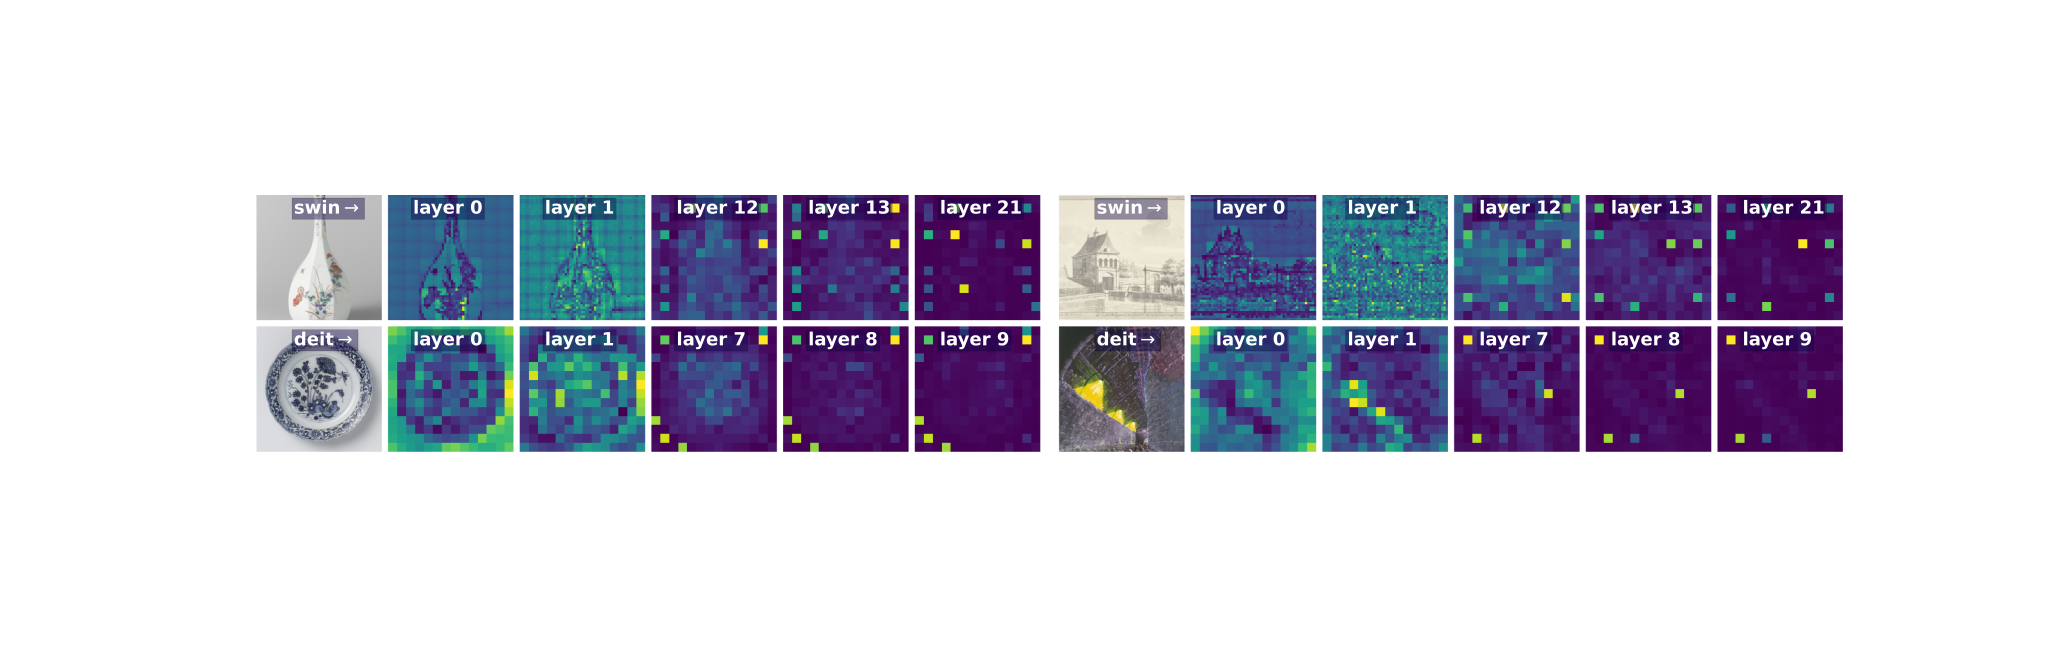
\includegraphics[width=\textwidth]{img/layers.png}
    \caption{Attention layers of successively deeper transformer blocks.}
    \label{results:img:layers}
\end{figure*}

\begin{figure*}[tb]
    \centering
    \begin{subfigure}{0.49\textwidth}
    \includegraphics[width=8cm]{img/img005_salience.png}
    \caption{Dish}
    \label{results:img:sal:dish}
    \end{subfigure}
    \begin{subfigure}{0.49\textwidth}
    \includegraphics[width=8cm]{img/img011_salience.png}
    \caption{Picture}
    \label{results:img:sal:dish}
    \end{subfigure}
    \caption{Examples of saliency maps for different models.}
\end{figure*}
